\documentclass[11pt]{article}
\usepackage{coling2014}
\usepackage{times}
\usepackage{url}
\usepackage{latexsym}
\usepackage{graphicx}
\usepackage{amsmath}
\usepackage{xcolor}

%\setlength\titlebox{5cm}

% You can expand the titlebox if you need extra space
% to show all the authors. Please do not make the titlebox
% smaller than 5cm (the original size); we will check this
% in the camera-ready version and ask you to change it back.


\title{Modelling of Adjectives in the Ontology-Lexicon Interface}

\author{John P. M\textsuperscript{c}Crae \\
  Affiliation / Address line 1 \\
  Affiliation / Address line 2 \\
  Affiliation / Address line 3 \\
  {\tt email@domain} \\\And
  Francesca Quattri, Chrisitina Unger, Philipp Cimiano \\
  Affiliation / Address line 1 \\
  Affiliation / Address line 2 \\
  Affiliation / Address line 3 \\
  {\tt email@domain} \\}

\date{}

\begin{document}
\maketitle
\begin{abstract}
    The ontology-lexicon interface has become an important and successful tool 
for handling problems in NLP. The foundation of these models based on the
separation of the ontological and lexical layers by means of the principle of 
semantics by reference to an ontology in description logics. However, as noted 
by other authors, the use of first order logic (hence also description logics),
while effective for nouns and verbs breaks down in the case of adjectives. 
We propose that this is primarily due to a lack of logical expressivity in the 
ontology. \textbf{In particular, many adjectives are i) gradable requiring fuzzy or 
non-monotonic semantics or ii) operator adjectives require second-order logic. \textcolor{blue}{What about all the other classes of adjectives that you propose in the paper?}}
We consider  how we can handle the ontology-lexicon interface in the face of 
these more complex logical formalism, and show how these can be backward 
engineered into OWL based modelling by means of pseudo-classes, with application
to question answering.
\end{abstract}



\section{Introduction}
\label{intro}
\blfootnote{  
     This work is licensed under a Creative Commons 
     Attribution 4.0 International Licence.
     Page numbers and proceedings footer are added by
     the organisers.
     Licence details:
     \url{http://creativecommons.org/licenses/by/4.0/}
}

Ontology-lexicon models, such as the \emph{lemon} (Lexicon Model for Ontologies)~
\cite{mccrae2012interchanging}, have become an important model for handling a 
number of tasks in natural language processing. In particular, such 
ontology-lexica are built around the separation of a lexical layer describing 
how a word or phrase acts syntactically\textbf{; a } morphology and a semantic layer 
describing how the meaning of a word is expressed in a formal logical model, 
such as the OWL (Web Ontology Language)~\cite{mcguinness2004owl}. It has been 
shown that this principle known as \emph{semantics by reference}~
\cite{buitelaar2010ontology} is an effective model that can be used in tasks 
such as question answering \cite{unger2011pythia} and natural language 
generation \cite{cimiano2013exploiting}. In particular, its suitability to the 
task is driven by the fact that the application of this model to answering questions 
based on the DBpedia \cite{auer2007dbpedia} knowledge base \textbf{requires mostly 
understanding the nouns and the verbs of the sentence\textit{if this is a statement by \cite{auer2007dbpedia} the citation should be shifted here}}. However, as has been 
shown by the Question Answering over Linked Data \cite[QALD]{lopez2013evaluating}
tasks there are many questions that can be asked over this database that require 
a deeper semantic understanding of the representation of language. For example, 
questions such as 

\begin{quote}
What is the highest mountain in Australia?
\end{quote}

require understanding of the semantics of `high' in a manner that goes beyond 
the model of OWL based on classes, properties and individuals. The answer given 
in the QALD dataset for this question is as follows

\begin{verbatim}
SELECT DISTINCT ?uri WHERE { 
  ?uri rdf:type dbo:Mountain . 
  ?uri dbo:locatedInArea res:Australia . 
  ?uri dbo:elevation ?elevation . 
} ORDER BY DESC(?elevation) LIMIT 1
\end{verbatim}

In particular, the interpretation of this question involves the understanding of 
how the word `high' relates to the property {\tt dbo:elevation} and how to 
express this semantics in a formal manner.

\textbf{It has been claimed that first-order logic and thus by extension description 
logics, such as OWL, ``fail decidedly when it comes to adjectives''
\cite{bankston2003modeling}\textcolor{blue}{This statement motivates the whole paper. Further on Bankston's conclusions}}. To this extent, we largely agree that the semantics 
of many adjectives are difficult or impossible to describe in first-order logic, 
however, from the point of view of the ontology-lexicon interface, the logical 
expressivity of the ontology is not a limiting factor. In fact, due to the 
separation of the lexical and ontology layers in a model such as \emph{lemon}, 
it is possible to express the meaning of words without worrying about the 
formalism used in the ontology. To this extent, we will first demonstrate that 
adjectives are in general a case where the use of description logics (DL) breaks down, 
and for which more sophisticated logical formalisms must be applied. We then 
consider to what extent this can be handled in the context of the 
ontology-lexicon, and introduce pseudo-classes, that is OWL classes with 
annotations, which we use to express the semantics of adjectives in a manner
that would allow reasoning with fuzzy, high-order models. To this extent, we base
our models on the previously introduced design patterns~\cite{mccrae2014design}
for modeling ontology-lexica. 
Finally, we show how these semantics can be helpful in practical applications 
of question answering over the DBpedia knowledge base.

\section{Classification of adjectives}

There are a number of classifications of adjectives, and first we will start 
with the most fundamental distinction of \emph{attributive} versus 
\emph{predicative} usage, that is the use of adjectives in noun phrases 
(``$X$ is a $A~N$'') versus as objects of the copula (``$X$ is $A$''). 
It should be noted that there are many adjectives for which only predicative or 
attributive usage is allowed.

\begin{quote}
	Clinton is a former president.
	
	$^*$Clinton is former.
	
	The baby is awake.
	
	$^*$The awake baby.
\end{quote}

\textbf{\textcolor{blue}{On Clinton: here it could be specified that ATTRIBUTIVE adjectives come in the first position (e.g. the blue sea, the old man), while PREDICATIVE adjectives follow a verb. While most adjectives can be both attributive and predicative, some can only take the attributive (e.g. the main reason, the former president) or only the predicative (e.g. *the awake baby, *the afraid child) position. 
Ref.\url{http://www.ucl.ac.uk/internet-grammar/adjectiv/attribut.html}}}One of the principle classifications of the semantics of adjectives (for example \cite{partee2003there,bouillon1999description}) is based on the meaning of adjective noun compounds relative to the meaning of the words by themselves. This classification is as follows (where $\Rightarrow$ means it entails)

\begin{description}
\item[Intersective] ($X\mathrm{~is~a~}A~N \Rightarrow X\mathrm{~is~}A \cap X\mathrm{~is~a~}N$) 
Such adjectives work as if they were another noun and indicate that the compound 
noun phrase is a member of both the class of the noun and the class of the 
adjective. For example, in the phrase ``Belgian violinist'' it refers to a 
person in the class intersection $Belgian \sqcap Violinist(X)$, \textbf{and hence we 
can infer that a ``Belgian violinist'' is a subclass of a ``Belgian person''.\textcolor{blue}{rather than ending the intersective session with this example (which would remind somebody of ontological order), you can conclude by saying "hence the inference "He is a Belgian surgeon" from "He is a Belgian violinist. He is a surgeon." is still valid.  Also: Here it could be further explained by saying, since the adjective 'skilful' does not maintain a kind of truth-conditional independence from the noun it combines with. 
Why I think Morzycki \cite{morzycki2013nonscales} explains it better than Partee \cite{partee2003there}: \url{https://www.msu.edu/~morzycki/work/papers/chapter_notscales.pdf}}}
\item[Subsective] ($X\mathrm{~is~a~}A~N \Rightarrow X\mathrm{~is~a~}N, X\mathrm{~is~a~}A~N \not\Rightarrow X\mathrm{~is~}A$) 
Such adjectives do not alter the meaning of the noun phrase itself, but only 
make sense with knowledge of the noun they refer to. For example, a ``\textbf{skilful\textit{btw, Collins acknowledges 'skilful' with one 'l' but all the examples i have found in literature report 'skillful' with two 'l's.}}
violinist'' is certainly in the class $Violinist(X)$, but if we knew that that 
person is a surgeon as well, we cannot conclude that the person is a skilful surgeon. 
\item[Privative] ($X\mathrm{~is~a~}A~N \not\Rightarrow X\mathrm{~is~a~}N$) 
These adjectives modify the meaning of a noun phrase \textbf{to create a noun phrase 
that is incompatible with the original meaning. For example, a 
``fake gun'' is not a member of the class of guns.\textcolor{blue}{Put in these terms, the definition of privative adjectives could also justify idiomatic expressions, such as big shot, which is transparently non-compositional. In fact, the meaning of the noun phrase is incompatible with the original meaning of its parts. What could be said here in the case of privative adjectives, is more that these adjectives are not just non-intersective (as in the case of 'alleged thief, where the person can or cannot be a thief), but anti-intersective, since the adjectives CAN'T (instead of don't) entail reference to the objects denoted by the noun. In 'a fake gun' the 'gun' in question cannot for sure be a gun.}}
\end{description}

This classification is useful, however one further case is important to 
distinguish and that is of \emph{relational} adjectives which have a meaning 
that expresses a relationship between two individuals or events, for example:

\begin{quote}
\textbf{I would rather go to the sea than the mountains.\textcolor{blue}{No adjective here. I would skip the example}}

\textbf{He is related to her.\textcolor{blue}{For an example for this class of adjectives, I would go back to Morzycki \cite{morzycki2013nonscales}. Some define 'relational' adjectives also 'classificatory' since they could be confused with 'relative'. McNally \& Boleda Torrent (2003) define them as adjectives that define properties of KINDS (e.g. a medical student, a technical architect, a religious official), where the adjective does not describe the person itself, but the KIND of person that is instantiated in the noun. }}
\end{quote}

Another important distinction to make with adjectives is whether they are 
\emph{gradable}, in that whether it makes semantic senses to make a comparative 
or superlative statement with these adjectives. For example, adjectives such as 
`big' or `tall' can express relationships such as `$X$ is bigger than $Y$', 
however it is not possible to say one individual is `more former'. \textbf{Most gradable 
adjectives are subsective, for example `a big mouse' is not `a big animal'.\textcolor{blue}{In case you need a citation for this statement: Morzycki (\cite{morzycki2013nonscales}:23; ex. (55) (56)): "the biggest classes of subsective adjectives are gradable"}} An 
important group of gradable adjectives are, however, intersective, and we call 
such adjectives `absolute' (following \cite{rusiecki1985adjectives}) as they 
refer to an ideal point on some scale, \textbf{for example a `dry towel' is `dry', in 
that it has little or no water, however we can still talk about a towel being 
`drier', in the sense of closer to the ideal of having no water than some other 
object.\textcolor{blue}{if the example of 'dry' poses a problem, since it seems to  be relative to the context of use, you can use adjectives like "triangular", "bent" or "straight" and justify that absoluteness either because their arguments already possess the maximum degree of the measured concept (e.g. "straight"), or because they require their arguments to possess a zero-degree of the relevant concept (as in the case of "bent"). Here i am citing (\cite{kennedy2007vagueness}:4)}}

Finally, we consider \emph{operator} or \emph{property-modifying} adjectives, 
which can be considered to be the same as privative adjectives, but in this 
case are understood as operators that change some property in the qualia 
structure of the class. For example, we may express the adjective `former' 
as follows in lambda calculus~\cite{partee2003there}:

$$\lambda C [\lambda x \exists t C(x,t) \cap t < \mathrm{now}]$$

Such adjectives have not only a difference in semantic meaning but can also 
frequently have syntactic impact, for example in adjective ordering 
restrictions, as they may be reordered with only semantic 
impact~\cite{teodorescu2006adjective}, e.g.,

\begin{quote}
A big red car.

\textbf{$^?$A red big car.\textcolor{blue}{Given the possibility that somebody criticizes this particular example claiming that that Teodorescu's example is weak since it is feasible to change the syntactic order of operator adjectives, I found a paper by Beck \cite{beck2000relational}. Instead of mentioned the exploration of Polish example by Partee (2003) below, you could directly take Berg's examples in German, where she analyzes anders and verschieden for 'different'. She claims that while verschieden is a relational adjective that induces a hidden reciprocal (e.d. Karl und Teo lesen verschiedene Buecher = Karl reads a different book from the book Teo is reading); anders is a comparison operator (Karl und Teo lesen andere Buecher = Karl und Teo read different books from the ones that are read by everyone else). From here derives that 'different' acts as relative and operator or property-modifying adjective. }}

A famous former actor.

A former famous actor.
\end{quote}

A related syntactic phenomena for Polish is explored by Partee \shortcite{partee2003there}.

\section{Representation of adjectives in the ontology-lexicon interface}

In general it is assumed that adjectives form frames with exactly one argument 
except for extra arguments given by adjuncts, typically prepositional phrases. 
Most adjectives are thus associated with a predicative frame, stereotyped in 
English as:

$$X\mathrm{~is~}A$$

And with a second attributive frame, whose stereotype is not directly 
realizable but we give as:

$$X [attr] A$$

As such, when we encounter the attributive usage of an adjective such as in

\begin{quote}
Juan is a Spanish researcher
\end{quote}

We understand this as the realization of two frames:

\begin{quote}
\textbf{Juan is a researcher.\textcolor{blue}{this point is tricky. Looks like you are mixing copula with attribute. Since later you just develop Belgian in LEMON, I'd leave this example out}}

Juan $[attr]$ Spanish.
\end{quote}

Note we do not provide modeling for adjectives that are part of a noun phrase,
such as `polar bear', which we would capture as a normal noun phrase with 
meaning \emph{ursus maritimus}.

\subsection{Intersective adjectives}

Intersective adjectives are the most straightforward class as in many cases they 
can mostly be explained as either being noun-like (denominal adjectives such as 
`British') or verb-like (deverbal adjectives such as `broken'). Intersective 
adjectives have a single argument as with most adjectives and in this case it is 
natural that they refer to classes, which may be event classes such as described 
in \cite{mccrae2014design}. For practical modeling examples we will use the
\emph{lemon} model as it is the most prominent implementation of the 
ontology-lexicon interface.

The primary mechanism of modelling the syntax-semantics interface in the context 
of \emph{lemon} is by means of assigning a \emph{frame} as a \emph{syntactic 
behaviour} of an entry and giving it \emph{syntactic arguments}, which can then 
be linked to the \emph{lexical sense}, which stands in proxy for a true semantic 
frame in the ontology. For example, the modelling of an adjective such as 
`Belgian' can be achieved as follows (depicted in figure 
\ref{example-belgian})\footnote{We assume that the namespaces are defined for 
the lexicon as {\tt lexicon}, e.g., \url{http://www.example.org/lexicon}
and for the entry, e.g., {\tt belgian} is \url{http://www.example.org/lexicon/belgian#},
other namespaces are assumed to be as usual.}.

\begin{figure}

\includegraphics[width=\textwidth]{belgian-example}
\caption{Modelling of an intersective adjective `Belgian' in \emph{lemon}\label{example-belgian}}
\end{figure}

\begin{verbatim}
lexicon:belgian a lemon:LexicalEntry ;
  lemon:canonicalForm belgian:Lemma ;
  lemon:synBehavior belgian:AttrFrame , 
                    belgian:PredFrame ;
  lemon:sense belgian:Sense .

belgian:Lemma lemon:writtenRep "Belgian"@eng .

belgian:AttrFrame lexinfo:attributiveArg belgian:AttrSynArg .

belgian:PredFrame lexinfo:copulativeArg belgian:PredSynArg .

belgian:sense lemon:reference [
    a owl:Restriction ;
    owl:onProperty dbpedia:nationality ;
    owl:hasValue dbpedia:Belgium ] ;
  lemon:isA belgian:AttrSynArg ; belgian:PredSynArg .
\end{verbatim}

Note, that here we use the external vocabulary LexInfo \cite{cimiano2011lexinfo} 
to define the meaning of the arguments of the frame as the \emph{attributive 
argument}, corresponding to the frame stereotype ``A $[attr]$ X'' and the 
\emph{copulative argument} for the frame stereotype ``X is an A''. Furthermore,
the class of Belgians is not named in our reference ontology DBpedia, so we 
introduce an anonymous class with the axiomatization, 
$\exists \text{nationality}.\text{Belgium}$. It is in fact common that the 
referent of an adjective is not named in an ontology and as such we tend to 
model denomial adjectives as the form $\exists \text{prop}.\text{Value}$, 
where $\text{Value}$ is the reference of the noun from which the adjective is
derived. This modelling is so common that it has already been encoded as two
patterns, called {\tt IntersectiveObjectPropertyAdjective} and {\tt
IntersectiveDatatypePropertyAdjective}, see McCrae and Unger \shortcite{mccrae2014design}.
Similarly, most deverbal adjectives refer to an event, and as such
a common modelling is of the form $\exists theme^{-1}.EventClass$, for example 
`vandalized' may be $\exists theme^{-1}.VandalismEvent$.

\subsection{Gradable adjectives}

\textbf{Gradable adjectives are naturally defined relative to a particular 
property\textcolor{blue}{Before introducing variant and covariant, a list of the properties of gradable adjectives could be introduced. For this, I am referring to two papers of Kennedy, \cite{kennedy1999scalar,
kennedy2007vagueness}).}}\footnote{Note in many cases the property is quite abstract such as in 
`breakable' \textbf{moar}}
\begin{itemize}
\item \textbf{\textcolor{blue}{the property of comparative constructions is only true in the case of gradable adjectives (\cite{kennedy1999scalar}:3); non-gradable adjectives are in fact anomalous in comparisons (e.\,g. 
`*less geological', `*more wooden' (\cite{kennedy2007vagueness}:22))}}
\item \textbf{\textcolor{blue}{the interpretation of gradable adjectives is very context-dependent (\cite{kennedy1999scalar}:4)}}
\item \textbf{\textcolor{blue}{\textit{relative} gradable adjectives, like `expensive', possess the feature of vagueness (\cite{kennedy2007vagueness}:3)}}
\item \textbf{\textcolor{blue}{\textit{absolute} gradable adjectives, like `straight' or `bent' or `red' (to cite your part on colors below), are not vague}}
\item \textbf{\textcolor{blue}{gradable adjectives have a context-dependent truth-conditional variability, meaning that their positive form is the sum of the relation between the degree of the concept possessed by the object (as measured by the predicate) and the context-dependent standard of comparison based on the same concept \cite{kennedy2007vagueness}. It follows that the properties denoted by adjectives like `expensive' or `small' or `big' vary in intensity according to the context (and time) of use. (at this place your example on `tall' could be introduced)}}
\item \textbf{\textcolor{blue}{the arguments of gradable adjectives are mapped into abstract representations of measurements or degrees, whereas a set of degrees constitutes a scale (\cite{kennedy2007vagueness}:4)}}
\item \textbf{\textcolor{blue}{Along with degrees and scales, one can also determine whether a gradable adjective (relative or absolute) has a minimum or a maximum standard. For instance, `transparent' has a maximum standard (complete transparency), while `opaque' has a minimum standard (partial visibility) (\cite{kennedy2007vagueness}:37). (This part could be added as well as left out; Kennedy (2007) claims that, apart from some exceptions, some closed scaled adjectives have fixed standards of comparisons (\cite{kennedy2007vagueness}:38), such as `closed', `hidden', `covered', while others have minimum standards, such as `acquainted with' (which is understandable), or `documented' (eben, not so clear why this has minimal standards))}}
\end{itemize}

, that is it is natural to say that \textbf{`big' refers to 
`size', however it is clear then that `small' also refers to `size' and as antonyms 
they cannot both refer to the same ontological concept.\textcolor{blue}{You introduce here a gradable adjective such as 'big' already in conjunction with its antonym 'small'. A further premise to 'big' (\cite{kennedy2007vagueness}:6) could be that 'big' is defined 'vague' as well as 'gradable' since it applies or measure distinct truth conditions. This could be included as example in the list above.}} \textbf{As such, we introduce 
the concept of \emph{covariance} and \emph{contravariance}, which refers to 
whether the comparative form indicates a higher property value for the subject 
or the object. That is that `big' is covariant with size, as bigger things have 
a higher size value, and `small' is contravariant with size.\textcolor{blue}{See my comment below.**}} \textbf{We also introduce 
a third concept of \emph{absolute gradability}, which states that these objects 
are better described by these adjectives as they approach some ideal value. \textcolor{blue}{If you want to use Kennedy's definitions of gradable adjectives, this part is already in the itemized list.}}
\textbf{A common example of this is colours, which where we may say that some object is 
redder than another if it is closer to some ideal value of red 
(e.g., RGB {\tt 0xff0000}).}

\textbf{\textcolor{blue}{On variant and covariant** MORE TO COME}}
  
\textbf{\textcolor{blue}{You introduce here the concepts of covariance and contravariance with reference to antonymic adjectives and the concept they refer to (e.\,g. `big' / `small' and `size'). MORE TO COME}}

While these concepts well handle the comparative usage of adjectives, the 
predicative and superlative usage of adjectives is complicated by three factors 
that we will outline below. Firstly, we notice that gradable classes are not 
crisply defined as with the case of many intersective adjectives, that is that 
while we can clearly define all people in the world as `British' or 
`non-British', by who holds a passport of the United Kingdom, it is not easy 
split the world's population into `tall' and `not tall'. In fact, while it may 
be easy to say that someone who is 6'6'' (198cm) tall is `tall' it is not clear 
whether someone of height 6' (182cm) is `tall' although they are above average 
height for a man. As such, the class boundary of a gradable adjective are 
naturally fuzzy. Secondly, we note that these class boundaries are 
non-monotonic, that is that with knowledge of more instances of the relative 
class we must revise our class boundaries. \textbf{This is especially the case for the
superlative as the discovery of a new tallest person in the world would remove 
the existing tallest person in the world from the class of tallest person in the 
world. This, non-monotonicity also affects the class boundaries of the gradable 
class itself, for example in the 18th century the average height of a male was 
5'5'' (165cm)\textcolor{blue}{This passage kind of reiterates what you have stated above.}}\footnote{\url{http://en.wikipedia.org/...}}
and as such a male of 6' would have been considered clearly to be 
tall. As such, we can conclude that each instance added to our ontology must 
revise the class boundaries of a gradable class, hence leading to the fact that 
gradable adjectives are fundamentally non-monotonic. Finally, we must notice 
that gradability can only be understood relative to the class that we wish to 
grade, that is that while it is unclear as to whether 6' is tall for a male, 
given the current average height of a female of about 5'4'' (162cm) it is clear 
that 6' is clearly tall for a female.

As such we can clearly conclude that gradable adjectives are \emph{fuzzy} and
\emph{non-monotonic} and \emph{context-sensitive}, all of which are incompatible 
with the description logic
used by OWL. Currently there are only limited models for representing fuzzy 
logic in the context of the web~\cite{zhao2008uncertainty}. As such, we 
introduce a new model, which we name \emph{lemonOILS} (The \emph{lemon} 
Ontology for the Interpretation of Lexical Semantics)
\footnote{\url{http://lemon-model.net/oils}}. This ontology introduces three 
new classes:

\begin{itemize}
	\item {\tt CovariantScalar}: Indicating that the adjective is covariant with its bound property
	\item {\tt ContravariantScalar}: As above, but contravariant
	\item {\tt AbsoluteScalar}: Indicating that the property represents similarity to an absolute value
\end{itemize}

In addition, the following properties are introduced to enable the description 
of gradable adjectives. Note, that all of these properties are typed as 
\emph{annotation properties} in the OWL ontology, so that they do not interfere 
with the standard OWL reasoning.

\begin{itemize}
	\item {\tt boundTo}: Indicates the property that a scalar refers to (e.g., `size' for `big')
	\item {\tt threshold}: A sensible minimal value by which the adjective can be said to hold.
	\item {\tt degree}: One of {\tt weak}, {\tt medium}, {\tt strong} or {\tt very strong} corresponding to approximately 50\%, 25\%, 5\% or 1\% of all known individuals.
	\item {\tt comparator}: Indicates an object property that is equivalent to the comparison of the adjective. e.g., an object property {\tt biggerThan} may be considered a comparator for the adjective class {\tt big}.
	\item {\tt measure} (TODO)
	\item {\tt defaultValue} (TODO)
\end{itemize}

Using such classes we can capture the semantics of gradable adjectives 
syntactically but not formally within an OWL model, as such we call such 
introduced classes \emph{pseudo-classes}. An example of modelling an adjective 
such as `high' is given below (figure \ref{high-example}).

\begin{figure}
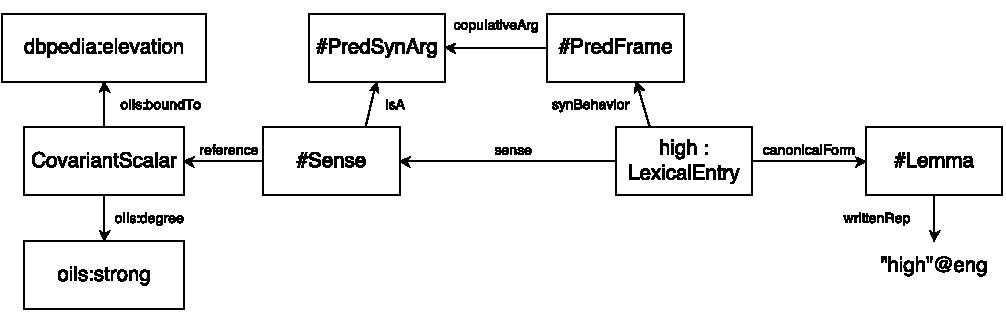
\includegraphics[width=\textwidth]{high-example}
\caption{An example of the modelling of `high' in \emph{lemon}\label{high-example}}
\end{figure}

\begin{verbatim}
lexicon:high a lemon:LexicalEntry ;
  lemon:canonicalForm high:Lemma ;
  lemon:synBehavior high:PredFrame ;
  lemon:sense high:Sense .

high:Lemma lemon:writtenRep "high"@eng .

high:PredFrame lexinfo:copulativeArg high:PredArg .

high:Sense lemon:reference [
    rdfs:subClassOf oils:CovariantScalar ;
    oils:boundTo dbpedia:elevation ;
    oils:degree oils:strong ] ;
  lemon:isA high:PredArg .
\end{verbatim}

As an example of a way in which it would be possible to interpret these 
annotations, we consider Markov Logic~\cite{richardson2006markov}, which is an 
extension of first-order logic in which each clause is given a cost. The process 
of reasoning is thus transformed into an optimization problem of finding the 
extension, which minimizes the summed weight of all violated clauses. As such we
can formulate a gradable adjective based on the number of known instances as 
follows:

$$\forall x \in C, y \in C : size(x) > size(y) \rightarrow big_C(x) : \alpha$$

$$\forall x \in C, y \in C : size(x) < size(y) \rightarrow \neg big_C(x) : \beta$$

Where the values of $\alpha$ and $\beta$ are related to the degree defined
in the ontology.
In this way, the classification of an object into big or small is defined as follows:

\noindent\textbf{Lemma}: An individual, $x \in C$, has $big_C(x)$ if and only if 

$$|\{y \in C, size(y) > size(x)\}| \alpha > |\{y \in C, size(y) < size(x)\}| \beta$$

The proof of this lemma is trivial, and we see the three properties clearly 
outlined above, in that we have non-monotonicity (in that more individuals may
 change whether we consider an individual to be `big' or not, that we have 
fuzziness, given by the strength of the probability of the proposition 
$big_C(x)$.

\textbf{Thresholds, defaults and multiple classes (Francesca to help)}

\subsection{Operator adjectives}

Operator adjectives are those that combine to alter the meaning of the adjective 
itself. There are two primary issues with the understanding of the adjective in 
this manner, firstly that the reference of the lexical item does not directly 
refer to an existing item in the ontology, but rather is novel and productive 
and secondly that the compositional nature of adjective-noun compounds is no 
longer simple as in the cases of intersective and gradable adjectives. This 
means that we must acknowledge operator adjectives in both the lexicon and the 
adjective. To this extent we define a frame known as the operator adjective 
frame, whose prototype is:

$$X\mathrm{~is~a~}A~NP$$

This leads to the odd case that operator adjectives are then considered the 
head of the frame! \textbf{hmm...} In this case 
we can understand the reference of the adjective as a property that relates an 
individual to a class. As such it is clear, that the reference of an operator 
adjective is a higher-order predicate. Fortunately, in the case of OWL we can 
cheat on this second-order nature by means of \emph{punning}, which allows a 
class to also be an individual. If we thus assume that operator adjectives are 
essentially puns, then it follows that we can assume that the reference of an 
operator adjective is thus a property. As such, for example, we can model an 
adjective such as `former' as referring to a property such as {\tt heldRole} 
whose range is a class of roles punned as individuals. This approach is 
effective, however it has limits in general \textbf{does it???}

We will not be able to easily create a vocabulary that can fully describe the 
semantics of the adjective within the context of OWL as the second nature order 
of the logic cannot be captured well within the framework of description logic. 
However, we can use the punning trick described above to capture the semantics
of the adjective. To do this we need to add a frame on the syntax side, that 
indicates that the argument of the adjective is in fact the noun phrase. We 
would do this as follows (figure \ref{former-example}):

\begin{figure}
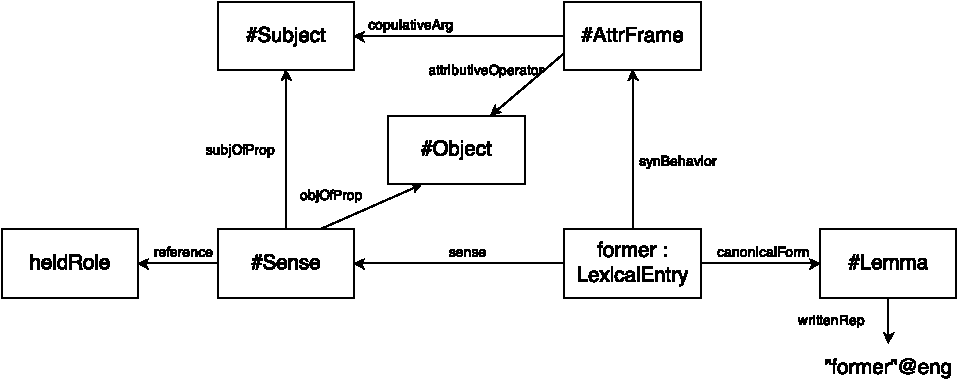
\includegraphics[width=\textwidth]{former-example}
\caption{An example of modelling `former' in \emph{lemon}\label{former-example}}
\end{figure}

\begin{verbatim}
former: a lemon:LexicalEntry ;
	lemon:canonicalForm former:Lemma ;
	lemon:synBehavior former:OperatorFrame ;
	lemon:sense former:Sense .

former:Lemma lemon:writtenRep "former"@eng .

former:OperatorFrame lexinfo:copulativeArg former:Subject ;
  lexinfo:attributiveOperator former:Object .
  
former:Sense lemon:reference onto:heldRole ;
  lemon:subjOfProp former:Subject ;
  lemon:objOfProp former:Object .
\end{verbatim}

The usage of this frame is intended such that a phrase such as:

\begin{quote}
Clinton is a former president
\end{quote}

Is interpreted as:

\begin{verbatim}
ontology:Clinton ontology:heldRole ontology:President .
\end{verbatim}

\subsection{Relational adjectives}

Relational adjectives are among the simplest and modelled with another frame,
which extends the attributive frame by allowing for a prepositional phrase
adjunct. As such we can model `known' with the frame `$X$ is known to $Y$' and
reference {\tt foaf:knows} as:

\begin{verbatim}
lexicon:known a lemon:LexicalEntry ;
  lemon:canonicalForm known:Lemma ;
	lemon:sense known:Sense ;
	lemon:synBehavior known:Frame .

known:Lemma lemon:writtenRep "known"@eng .

known:Frame lexinfo:attributeArg known:Subject ;
  lexinfo:prepositionalObject known:Object .

known:Sense lemon:reference foaf:knows ;
  lemon:subjOfProp known:Subject ;
	lemon:objOfProp known:Object .
	
known:Object lemon:marker lexicon:to .
\end{verbatim}

\section{Adjectives in question answering}

(Christina, some examples for QALD)

QALD, questions with adjectives:

What is the second highest mountain on Earth?

Who is the youngest player in the Premier League?

What is the longest river?

Give me all cars that are produced in Germany.

How tall is Michael Jordan?

Give me all Danish films.

How high is the Mount Everest?

What is the largest city in Australia?

In which city was the former Dutch queen Juliana buried?

Is Egypts largest city also its capital?

Who wrote the lyrics for the Polish national anthem?

Which mountain is the highest after the Annapurna?

Give me all communist countries.

Which U.S. state has the highest population density?

What is the highest mountain in Australia?

Is Frank Herbert still alive?

What is the highest place of the Urals?

Which mountains are higher than the Nanga Parbat?

Who was the first president of the United States?

What is the highest mountain?

Which budget did the first movie of Zdenek Sverak have?

Is Jens Friebe a vegan?

What is the most beautiful painting?

\section{Related work}

The categorization of adjectives in terms of formal semantics goes back to Montague\shortcite{montague1970english} and Vendler\shortcite{vendler1968adjectives}, however one of the most significant attempts to assign a formal meaning was carried out in the Mikrokosmos project\cite{raskin1995lexical}. This was one of the first works to treat the case of a micro-theory of adjectives, in which the results were ``machine-tractable'', in that they could be formally defined by a computer. The applications of this were limited however and no formal logic was attached to the semantic representations, nevertheless much of the modelling resembles ours. In particular, scalar adjectives are modelled by association with an attribute and a range, e.g., `big' was described as being {\tt >0.75} (i.e., 75\% of all known instances) on the {\tt size-attribute}. These classifications do not however clearly separate meaning and syntax and as they also required a seperate modelling of comparatives and class-specific meanings for many adjectives.

Amoia and Garden~\shortcite{amoia2006adjective} handled the problem of adjectives in the context of textual entailment and they analyzed 15 classes that show the subtle interaction between the semantic class (e.g., `privative') and the issues of attributive/predicative use and gradability. 

Abdullah and Frost~\shortcite{abdullah2005adjectives} tackles the privative nature of adjectives by arguing that the adjectives modify the set themselves, in a manner that is naturally second-order. Similarly, Partee~\shortcite{partee2003there} proposed a limited second-order model by means of their `head primary principle' requiring that adjectives are interpreted within their context. The analysis of Bankston~\shortcite{bankston2003modeling} however shows that the fundamental nature of many adjectives is higher-order, and provides a very sophisticated formal representation framework for this syntactic class.

The Generative Lexicon~\cite{pustejovsky1991generative} provides another approach to the representation of semantics, and the case of adjectives has also been considered in this context. Bouillion~\shortcite{bouillon1999adjective} consider the case of the French adjective `vieux' (`old') and...

Peters and Peters~\shortcite{peters2000treatment} provide one of the few other practical reports on modelling adjectives with ontologies, in the context of the SIMPLE lexica. This work is primarily focussed on the categorization of by means of intensional and extensional properties, rather than due to their logical modelling. 

\section{Conclusion}

In this paper we have presented a method for modelling adjectives with the
ontology-lexicon model, \emph{lemon}. In particular, we found that adjectives
frequently go beyond the first-order logic model used by OWL, but instead 
require models that are non-monotonic, fuzzy and second-order. As such, we 
conclude that more sophisticated semantic models are required to represent the semantics
of such words, however the separation of syntax and semantics remains a robust
model, which can easily be adapted to the task of representing adjectives. As 
a final note we consider the fact that not all languages even have adjectives
\cite{?} and as such we must wonder to what extent this analysis is applicable
beyond English. We contend, that the underlying semantics of the words we discuss here
is representable in all nearly languages and based on our analysis of realistic
questions as applied in QALD, we believe that this model should be applicable
to a range of domains and languages with little issue, however further 
validation is naturally necessary.

\section*{Acknowledgements}

\bibliographystyle{acl}
\bibliography{cogalex-adjectives}

\end{document}
